% ============================================================
%  Twittus_Extractorium --- Project Documentation
%  Modern LaTeX -- XeLaTeX recommended
% ============================================================
\documentclass[11pt, a4paper]{article}

% -- Core layout ---------------------------------------------
\usepackage[
  top=25mm, bottom=28mm,
  left=22mm, right=22mm,
  headheight=22pt
]{geometry}

% -- Typography -----------------------------------------------
\usepackage[expansion=false]{microtype}
\usepackage[T1]{fontenc}
\usepackage{setspace}
\setstretch{1.12}

% -- Colour palette -------------------------------------------
\usepackage[dvipsnames,table]{xcolor}
\definecolor{TwBlue}     {HTML}{1DA1F2}   % Twitter sky-blue
\definecolor{TwDark}     {HTML}{0D1117}   % near-black
\definecolor{TwMid}      {HTML}{1A2535}   % deep slate
\definecolor{TwAccent}   {HTML}{29AAE1}   % lighter blue
\definecolor{TwGray}     {HTML}{8B98A5}   % muted text
\definecolor{TwLight}    {HTML}{EAF4FB}   % pale blue fill
\definecolor{TwGreen}    {HTML}{17BF63}   % success
\definecolor{TwRed}      {HTML}{E0245E}   % warning / danger
\definecolor{TwYellow}   {HTML}{FFAD1F}   % caution
\definecolor{CodeBG}     {HTML}{F6F8FA}   % code background
\definecolor{CodeBorder} {HTML}{D0D7DE}   % code border

% -- Graphics & TikZ ------------------------------------------
\usepackage{tikz}
\usetikzlibrary{shapes.geometric, arrows.meta, positioning, calc, backgrounds}

% -- tcolorbox ------------------------------------------------
\usepackage{tcolorbox}
\tcbuselibrary{skins, breakable, listings}

% -- Code listings --------------------------------------------
\usepackage{listings}

\lstdefinestyle{pycode}{
  language=Python,
  backgroundcolor=\color{CodeBG},
  basicstyle=\ttfamily\footnotesize,
  keywordstyle=\color{TwBlue}\bfseries,
  commentstyle=\color{TwGray}\itshape,
  stringstyle=\color{TwGreen},
  numberstyle=\tiny\color{TwGray},
  breaklines=true,
  numbers=left,
  numbersep=8pt,
  frame=none,
  showstringspaces=false,
  tabsize=4,
  xleftmargin=6pt,
}

\lstdefinestyle{bashcode}{
  language=bash,
  backgroundcolor=\color{TwDark},
  basicstyle=\ttfamily\footnotesize\color{white},
  keywordstyle=\color{TwAccent}\bfseries,
  commentstyle=\color{TwGray}\itshape,
  stringstyle=\color{TwGreen},
  breaklines=true,
  frame=none,
  showstringspaces=false,
  tabsize=2,
  xleftmargin=6pt,
}

% tcolorbox styles for code
\tcbset{
  pybox/.style={
    enhanced, breakable,
    colback=CodeBG, colframe=CodeBorder,
    boxrule=0.6pt, arc=4pt,
    left=4pt, right=4pt, top=4pt, bottom=4pt,
    listing only,
    listing options={style=pycode},
    fonttitle=\bfseries\small\color{TwMid},
    attach boxed title to top left={yshift=-2mm, xshift=6mm},
    boxed title style={colback=TwBlue!15, colframe=TwBlue, arc=3pt, boxrule=0.5pt}
  },
  bashbox/.style={
    enhanced, breakable,
    colback=TwDark, colframe=TwMid,
    boxrule=0.6pt, arc=4pt,
    left=4pt, right=4pt, top=4pt, bottom=4pt,
    listing only,
    listing options={style=bashcode},
    fonttitle=\bfseries\small\color{TwGray},
    attach boxed title to top left={yshift=-2mm, xshift=6mm},
    boxed title style={colback=TwMid, colframe=TwGray, arc=3pt, boxrule=0.5pt}
  },
}

% -- Info / warning / tip boxes -------------------------------
\newenvironment{infobox}[1][Info]{%
  \begin{tcolorbox}[enhanced, breakable,
    colback=TwLight, colframe=TwBlue,
    boxrule=0.8pt, arc=5pt,
    left=8pt, right=8pt, top=5pt, bottom=5pt,
    title={\textbf{#1}},
    fonttitle=\small\color{TwBlue},
    attach boxed title to top left={yshift=-2mm, xshift=8mm},
    boxed title style={colback=TwLight, colframe=TwBlue, arc=3pt}]
}{\end{tcolorbox}}

\newenvironment{warnbox}[1][Warning]{%
  \begin{tcolorbox}[enhanced, breakable,
    colback=TwRed!6, colframe=TwRed,
    boxrule=0.8pt, arc=5pt,
    left=8pt, right=8pt, top=5pt, bottom=5pt,
    title={\textbf{#1}},
    fonttitle=\small\color{TwRed},
    attach boxed title to top left={yshift=-2mm, xshift=8mm},
    boxed title style={colback=TwRed!6, colframe=TwRed, arc=3pt}]
}{\end{tcolorbox}}

\newenvironment{tipbox}[1][Tip]{%
  \begin{tcolorbox}[enhanced, breakable,
    colback=TwGreen!8, colframe=TwGreen,
    boxrule=0.8pt, arc=5pt,
    left=8pt, right=8pt, top=5pt, bottom=5pt,
    title={\textbf{#1}},
    fonttitle=\small\color{TwGreen!70!black},
    attach boxed title to top left={yshift=-2mm, xshift=8mm},
    boxed title style={colback=TwGreen!8, colframe=TwGreen, arc=3pt}]
}{\end{tcolorbox}}

% -- Tables ---------------------------------------------------
\usepackage{booktabs}
\usepackage{tabularx}
\usepackage{array}
\usepackage{longtable}

% -- Headers & footers ----------------------------------------
\usepackage{fancyhdr}
\pagestyle{fancy}
\fancyhf{}
\fancyhead[L]{\small\color{TwGray}\textbf{Twittus\_Extractorium} \textnormal{--- Technical Documentation}}
\fancyhead[R]{\small\color{TwGray}v1.0}
\fancyfoot[C]{\small\color{TwGray}\thepage}
\renewcommand{\headrulewidth}{0.4pt}
\renewcommand{\headrule}{\hbox to\headwidth{\color{TwBlue!40}\leaders\hrule height\headrulewidth\hfill}}
\renewcommand{\footrulewidth}{0pt}

% -- Section styling ------------------------------------------
\usepackage{titlesec}
\titleformat{\section}
  {\large\bfseries\color{TwMid}}
  {\color{TwBlue}\S\thesection}{0.6em}{}[{\color{TwBlue!30}\titlerule[0.5pt]}]

\titleformat{\subsection}
  {\normalsize\bfseries\color{TwMid}}
  {\color{TwBlue}\thesubsection}{0.5em}{}

\titleformat{\subsubsection}
  {\small\bfseries\color{TwGray}}
  {\thesubsubsection}{0.4em}{}

\titlespacing{\section}{0pt}{16pt}{6pt}
\titlespacing{\subsection}{0pt}{10pt}{4pt}

% -- Hyperlinks -----------------------------------------------
\usepackage{hyperref}
\hypersetup{
  colorlinks=true,
  linkcolor=TwBlue,
  urlcolor=TwAccent,
  citecolor=TwBlue,
  pdftitle={Twittus\_Extractorium Documentation},
  pdfauthor={Twittus\_Extractorium Project},
  pdfsubject={Twitter/X Web Scraper Technical Documentation},
}
\pdfstringdefDisableCommands{%
  \def\cls#1{#1}%
  \def\method#1{#1}%
  \def\param#1{#1}%
  \def\pytype#1{#1}%
  \def\returns#1{Returns: #1}%
  \def\texttt#1{#1}%
  \def\color#1{}%
}

% -- Misc -----------------------------------------------------
\usepackage{enumitem}
\usepackage{parskip}
\setlength{\parskip}{5pt}
\raggedbottom
\usepackage{mdframed}
\usepackage{graphicx}
\usepackage{float}

% -- Helper macros --------------------------------------------
\newcommand{\badge}[2]{%
  \tikz[baseline=(n.base)]\node[
    fill=#1!18, draw=#1!60, rounded corners=3pt,
    inner xsep=5pt, inner ysep=2pt, font=\tiny\bfseries\color{#1!80!black}
  ](n){#2};%
}
\newcommand{\method}[1]{\texttt{\color{TwBlue}#1}}
\newcommand{\param}[1]{\texttt{\color{TwGreen!70!black}#1}}
\newcommand{\cls}[1]{\texttt{\color{TwMid}\textbf{#1}}}
\newcommand{\pytype}[1]{\texttt{\color{TwGray}#1}}
\newcommand{\returns}[1]{\textbf{Returns:} \texttt{#1}}

% ============================================================
\begin{document}
% ============================================================

% -- Cover / Title Page ---------------------------------------
\thispagestyle{empty}

\begin{tikzpicture}[remember picture, overlay]
  % Dark header band
  \fill[TwDark] (current page.north west)
    rectangle ([yshift=-72mm]current page.north east);
  % Blue accent stripe
  \fill[TwBlue] ([yshift=-72mm]current page.north west)
    rectangle ([yshift=-75mm]current page.north east);
  % Subtle circuit-dot decoration
  \foreach \x in {1,2,...,30}{
    \pgfmathsetmacro{\xx}{\x * 13.9}
    \fill[white, opacity=0.04] (\xx pt - 15cm, -12pt) circle (1.2pt);
  }
\end{tikzpicture}

\vspace*{20mm}

{\centering
  {\fontsize{9}{11}\selectfont\color{TwBlue}\textbf{\MakeUppercase{Technical Documentation}}}\\[4mm]
  {\fontsize{28}{32}\selectfont\bfseries\color{white}%
    \texttt{Twittus\_Extractorium}}\\[3mm]
\vspace{6mm}
  \badge{TwBlue}{Python 3.8+}\quad
  \badge{TwGreen}{Playwright}\quad
  \badge{TwYellow}{SQLite}\quad
  \badge{TwRed}{Ethical Use Only}\\[10mm]
  {\small\color{TwGray}Version \textbf{1.0} \quad|\quad \today}
\par}

\vspace{22mm}

% -- Abstract card --------------------------------------------
\begin{tcolorbox}[
  enhanced,
  colback=TwLight, colframe=TwBlue,
  boxrule=0.8pt, arc=6pt,
  left=10pt, right=10pt, top=8pt, bottom=8pt
]
\textbf{Abstract.}\quad
\textit{Twittus\_Extractorium} is a browser-automation-based scraper for
collecting publicly accessible tweets from X (formerly Twitter).
Built on \textbf{Playwright} and \textbf{SQLite}, it supports profile scraping,
keyword search scraping, deduplication, and human-like rate limiting.
It is intended exclusively for academic research, public-data analysis,
and journalistic investigation of publicly posted content.
\end{tcolorbox}

\vspace{6mm}

\begin{center}
\small\color{TwGray}
\begin{tabular}{ll}
\textbf{Language}   & Python 3.8 or later \\
\textbf{Browser engine} & Chromium via Playwright \\
\textbf{Storage}    & SQLite (file-based, zero server required) \\
\textbf{License}    & For research/academic use only \\
\end{tabular}
\end{center}

\newpage

% -- Table of Contents ----------------------------------------
\tableofcontents

\newpage

% ============================================================
\section{Introduction}
% ============================================================

\textbf{Twittus\_Extractorium} was designed to fill a pragmatic gap in social-media
research tooling: the official X API is rate-limited, expensive, and restricted,
yet a large body of publicly accessible content exists that researchers legitimately
need to study.

The scraper automates a real Chromium browser session through Playwright, closely
mimicking human browsing behaviour --- including randomised delays, gradual scrolling,
and a visible (non-headless) browser window --- to gather tweet metadata without
relying on undocumented API endpoints.

\subsection{Goals}

\begin{itemize}[leftmargin=1.6em, itemsep=3pt]
  \item Provide a single-login, multi-task batch scraping workflow.
  \item Store results in a local, portable SQLite database with automatic deduplication.
  \item Expose a clean Python API so downstream analysis scripts can invoke scraping as a library call.
  \item Maintain ethical use through rate-limiting, public-content-only access, and clear user disclaimers.
\end{itemize}

\subsection{Non-Goals}

\begin{warnbox}[Scope Limitations]
Twittus\_Extractorium does \textbf{not}:
\begin{itemize}[leftmargin=1.2em, itemsep=2pt]
  \item Access private accounts, DMs, or any content requiring special credentials.
  \item Bypass CAPTCHA or authentication challenges programmatically.
  \item Operate without a human confirming the login step.
  \item Support headless operation (headless mode cannot complete manual login).
\end{itemize}
\end{warnbox}

% ============================================================
\section{Architecture Overview}
% ============================================================

\subsection{Component Diagram}

\begin{figure}[H]
\centering
\resizebox{\textwidth}{!}{%
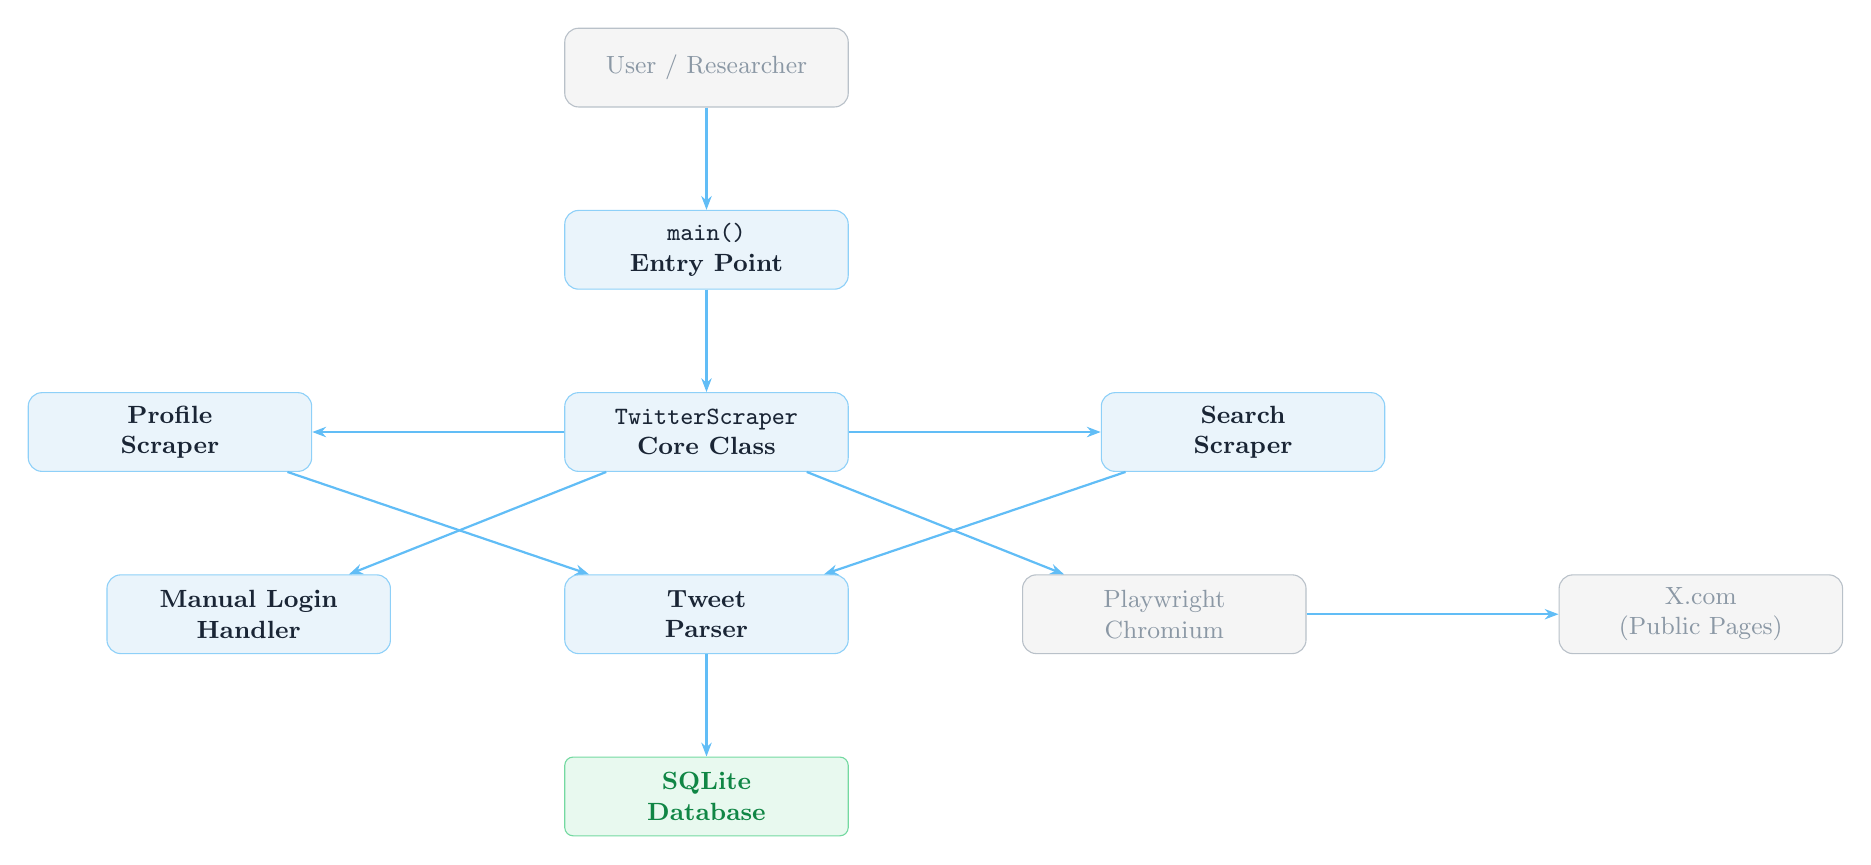
\begin{tikzpicture}[
  box/.style={draw=TwBlue!50, fill=TwLight, rounded corners=5pt,
              minimum width=36mm, minimum height=10mm,
              font=\small\bfseries, text=TwMid, align=center},
  db/.style={draw=TwGreen!60, fill=TwGreen!10, rounded corners=3pt,
             minimum width=36mm, minimum height=10mm,
             font=\small\bfseries, text=TwGreen!70!black, align=center},
  ext/.style={draw=TwGray!60, fill=gray!8, rounded corners=5pt,
              minimum width=36mm, minimum height=10mm,
              font=\small, text=TwGray, align=center},
  arr/.style={-{Stealth[length=5pt]}, TwBlue!70, thick},
  node distance=13mm and 22mm
]
  \node[ext]  (user)   {User / Researcher};
  \node[box]  (main)   [below=of user]    {\texttt{main()}\\Entry Point};
  \node[box]  (scraper)[below=of main]    {\cls{TwitterScraper}\\Core Class};
  \node[box]  (login)  [below left=of scraper]  {Manual Login\\Handler};
  \node[box]  (profile)[left=32mm of scraper]   {Profile\\Scraper};
  \node[box]  (search) [right=32mm of scraper]  {Search\\Scraper};
  \node[box]  (parser) [below=of scraper]       {Tweet\\Parser};
  \node[db]   (db)     [below=of parser]        {SQLite\\Database};
  \node[ext]  (pw)     [below right=of scraper] {Playwright\\Chromium};
  \node[ext]  (x)      [right=32mm of pw]       {X.com\\(Public Pages)};

  \draw[arr] (user)    -- (main);
  \draw[arr] (main)    -- (scraper);
  \draw[arr] (scraper) -- (login);
  \draw[arr] (scraper) -- (profile);
  \draw[arr] (scraper) -- (search);
  \draw[arr] (profile) -- (parser);
  \draw[arr] (search)  -- (parser);
  \draw[arr] (parser)  -- (db);
  \draw[arr] (scraper) -- (pw);
  \draw[arr] (pw)      -- (x);
\end{tikzpicture}}%
\caption{High-level component interaction for \textit{Twittus\_Extractorium}.}
\end{figure}

\subsection{Data Flow}

\begin{enumerate}[leftmargin=1.8em, itemsep=4pt]
  \item The user defines a list of \textbf{tasks} (profile scrapes and/or keyword searches).
  \item A single Chromium browser instance is launched; the user logs in manually.
  \item For each task, the scraper navigates to the target URL.
  \item Playwright locates \texttt{article[data-testid="tweet"]} elements.
  \item Each element is parsed by \method{parse\_tweet()} into a structured dictionary.
  \item New records are persisted to SQLite via \method{save\_tweets()}; duplicates are silently skipped.
  \item Human-like delays are injected between scrolls and between tasks.
\end{enumerate}

% ============================================================
\section{Installation \& Requirements}
% ============================================================

\subsection{Prerequisites}

\begin{center}
\begin{tabular}{lll}
\toprule
\textbf{Dependency} & \textbf{Version} & \textbf{Purpose} \\
\midrule
\rowcolor{TwLight} Python  & >= 3.8  & Runtime \\
playwright                 & >= 1.40 & Browser automation \\
\rowcolor{TwLight} Chromium browser & (via playwright install) & Page rendering \\
SQLite                     & bundled with Python & Data persistence \\
\bottomrule
\end{tabular}
\end{center}

\subsection{Step-by-Step Setup}

\begin{tcolorbox}[bashbox, title=1 --- Create a virtual environment]
\begin{lstlisting}[style=bashcode]
python -m venv .venv
source .venv/bin/activate        # Windows: .venv\Scripts\activate
\end{lstlisting}
\end{tcolorbox}

\begin{tcolorbox}[bashbox, title=2 --- Install Python dependencies]
\begin{lstlisting}[style=bashcode]
pip install playwright
\end{lstlisting}
\end{tcolorbox}

\begin{tcolorbox}[bashbox, title=3 --- Install Playwright browser binaries]
\begin{lstlisting}[style=bashcode]
playwright install chromium
\end{lstlisting}
\end{tcolorbox}

\begin{tcolorbox}[bashbox, title=4 --- Run the scraper]
\begin{lstlisting}[style=bashcode]
python twittus_extractorium.py
\end{lstlisting}
\end{tcolorbox}

\begin{tipbox}[Virtual Environment]
Always activate the virtual environment before running the scraper.
The script will fail silently if Playwright cannot find the Chromium binary.
\end{tipbox}
\newpage
% ============================================================
\section{Module Reference}
% ============================================================

\subsection{\texorpdfstring{Class \cls{TwitterScraper}}{Class TwitterScraper}}

The main class that orchestrates the browser session, scraping logic, and
database persistence. All public methods are described below.

\subsubsection{\texorpdfstring{Constructor}{Constructor}}

\begin{tcolorbox}[pybox, title={\texttt{\_\_init\_\_}}]
\begin{lstlisting}[style=pycode]
def __init__(self, db_path: str = "twitter_data.db",
             headless: bool = False)
\end{lstlisting}
\end{tcolorbox}

\begin{center}
\rowcolors{2}{TwLight}{white}
\begin{tabularx}{\linewidth}{llX}
\toprule
\textbf{Parameter} & \textbf{Type} & \textbf{Description} \\
\midrule
\param{db\_path}  & \pytype{str}  & File path for the SQLite database. Created automatically if absent. \\
\param{headless}  & \pytype{bool} & Must be \texttt{False} for manual login. Headless mode is incompatible with interactive login. \\
\bottomrule
\end{tabularx}
\end{center}

\subsubsection{\texorpdfstring{\method{wait\_for\_manual\_login(page)}}{\detokenize{wait_for_manual_login(page)}}}

Navigates to the X login page and pauses execution until the user presses
\texttt{ENTER} in the console. Performs post-login verification by checking
for multiple DOM indicators (primary column, account switcher, post button).

\returns{bool} --- \texttt{True} if login is confirmed, \texttt{False} otherwise.

\subsubsection{\texorpdfstring{\method{setup\_database()}}{\detokenize{setup_database()}}}

Creates the \texttt{tweets} table and two indices (\texttt{author\_username},
\texttt{scraped\_at}) if they do not already exist.

\subsubsection{\texorpdfstring{\method{save\_tweets(tweets)}}{\detokenize{save_tweets(tweets)}}}

\begin{tcolorbox}[pybox, title={\texttt{save\_tweets}}]
\begin{lstlisting}[style=pycode]
def save_tweets(self, tweets: List[Dict]) -> None
\end{lstlisting}
\end{tcolorbox}

Inserts tweet records into the database using \texttt{INSERT OR IGNORE} to
prevent duplicates keyed on \texttt{tweet\_id}. Logs counts of new saves and
skipped duplicates.

\subsubsection{\texorpdfstring{\method{human\_delay(min\_seconds, max\_seconds)}}{\detokenize{human_delay(min_seconds, max_seconds)}}}

Sleeps for a random duration drawn uniformly from
\texttt{[min\_seconds, max\_seconds]}. Default window is \textbf{1.5 -- 4.0 s}.

\subsubsection{\texorpdfstring{\method{scroll\_page(page, scrolls)}}{\detokenize{scroll_page(page, scrolls)}}}

Scrolls the page \param{scrolls} times by a randomised pixel offset
(500 -- 900 px per scroll), waiting 1.5 -- 3.0 s between each to allow
lazy-loaded content to appear.

\subsubsection{\texorpdfstring{\method{extract\_number(text)}}{\detokenize{extract_number(text)}}}

Converts human-readable engagement counts (\texttt{"1.2K"}, \texttt{"500"},
\texttt{"1M"}) to integers. \returns{int}

\subsubsection{\texorpdfstring{\method{extract\_tweet\_id(url)}}{\detokenize{extract_tweet_id(url)}}}

Parses the tweet ID from a status URL via the regex
\texttt{/status/(\textbackslash d+)}. \returns{Optional[str]}

\subsubsection{\texorpdfstring{\method{parse\_tweet(article\_element, source\_type, source\_query)}}{\detokenize{parse_tweet(article_element, source_type, source_query)}}}

The core extraction routine. Given a Playwright element handle for a tweet
\texttt{<article>}, it extracts:

\begin{itemize}[leftmargin=1.6em, itemsep=3pt]
  \item Tweet URL and ID (via \texttt{<time>} ancestor link)
  \item Author username (from URL path)
  \item Display name (first non-\texttt{@} span inside \texttt{[data-testid="User-Name"]})
  \item Tweet text (\texttt{[data-testid="tweetText"]})
  \item Engagement counts: likes, replies, retweets (from \texttt{aria-label} attributes)
  \item ISO 8601 timestamp (\texttt{<time datetime>})
\end{itemize}

\returns{Optional[Dict]} --- returns \texttt{None} if the element cannot be parsed.

\subsubsection{\texorpdfstring{\method{scrape\_profile(username, max\_scrolls, ...)}}{\detokenize{scrape_profile(username, max_scrolls, ...)}}}

\begin{tcolorbox}[pybox, title={\texttt{scrape\_profile}}]
\begin{lstlisting}[style=pycode]
def scrape_profile(
    self,
    username: str,
    max_scrolls: int = 5,
    page: Page = None,
    context = None,
    browser = None
) -> List[Dict]
\end{lstlisting}
\end{tcolorbox}

Navigates to \texttt{https://x.com/\{username\}} and collects tweets across
\param{max\_scrolls} scroll cycles.  Detects inaccessible profiles
(suspended/non-existent) before scraping.

\begin{center}
\rowcolors{2}{TwLight}{white}
\begin{tabular}{lll}
\toprule
\textbf{Parameter}    & \textbf{Default} & \textbf{Notes} \\
\midrule
\param{username}      & ---         & Without the \texttt{@} prefix \\
\param{max\_scrolls}  & \texttt{5} & Each scroll fires 2 sub-scrolls \\
\param{page}          & \texttt{None} & Pass an existing page to reuse session \\
\param{context}       & \texttt{None} & Pass for session reuse \\
\param{browser}       & \texttt{None} & Pass for session reuse \\
\bottomrule
\end{tabular}
\end{center}

\subsubsection{\texorpdfstring{\method{scrape\_search(query, max\_scrolls, ...)}}{\detokenize{scrape_search(query, max_scrolls, ...)}}}

Analogous to \method{scrape\_profile} but navigates to the URL
\texttt{https://x.com/search} with parameters \texttt{q} and
\texttt{f=live} (live/latest tab). The query is URL-encoded via
\texttt{urllib.parse.quote}.

\subsubsection{\texorpdfstring{\method{scrape\_with\_single\_login(tasks)}}{\detokenize{scrape_with_single_login(tasks)}}}

\begin{tcolorbox}[pybox, title={\texttt{scrape\_with\_single\_login}}]
\begin{lstlisting}[style=pycode]
def scrape_with_single_login(self, tasks: List[Dict]) -> None
\end{lstlisting}
\end{tcolorbox}

The recommended entry-point for batch usage. Launches a single browser,
performs one login, then iterates over all tasks, calling either
\method{scrape\_profile} or \method{scrape\_search} depending on the
task's \texttt{type} key.

\textbf{Task schema:}

\begin{center}
\rowcolors{2}{TwLight}{white}
\begin{tabular}{lll}
\toprule
\textbf{Key}         & \textbf{Type}  & \textbf{Values} \\
\midrule
\texttt{type}        & \pytype{str}   & \texttt{"profile"} or \texttt{"search"} \\
\texttt{target}      & \pytype{str}   & Username (no \texttt{@}) or search term \\
\texttt{max\_scrolls} & \pytype{int}  & Any positive integer (default \texttt{5}) \\
\bottomrule
\end{tabular}
\end{center}

% ============================================================
\section{Database Schema}
% ============================================================

All scraped data is stored in a single SQLite database file
(default: \texttt{twitter\_data.db}).

\subsection{Table: \texttt{tweets}}

\begin{center}
\rowcolors{2}{TwLight}{white}
\begin{tabularx}{\linewidth}{llX}
\toprule
\textbf{Column}            & \textbf{Type}    & \textbf{Description} \\
\midrule
\texttt{tweet\_id}         & TEXT (PK)        & Unique numeric ID extracted from tweet URL \\
\texttt{author\_username}  & TEXT             & Twitter handle (without \texttt{@}) \\
\texttt{author\_display\_name} & TEXT         & Display name as shown on the profile \\
\texttt{tweet\_text}       & TEXT             & Full plaintext body of the tweet \\
\texttt{tweet\_url}        & TEXT             & Canonical URL (\texttt{https://x.com/...}) \\
\texttt{like\_count}       & INTEGER          & Parsed like count at time of scrape \\
\texttt{reply\_count}      & INTEGER          & Parsed reply count \\
\texttt{retweet\_count}    & INTEGER          & Parsed retweet count (includes quote-tweets) \\
\texttt{timestamp}         & TEXT             & ISO 8601 original post time \\
\texttt{scraped\_at}       & TEXT             & ISO 8601 scrape timestamp \\
\texttt{source\_type}      & TEXT             & \texttt{"profile"} or \texttt{"search"} \\
\texttt{source\_query}     & TEXT             & Username or search query that yielded the tweet \\
\bottomrule
\end{tabularx}
\end{center}

\subsection{Indices}

\begin{itemize}[leftmargin=1.6em]
  \item \texttt{idx\_author\_username} on \texttt{author\_username} --- fast per-user queries.
  \item \texttt{idx\_scraped\_at} on \texttt{scraped\_at} --- fast recency-based queries.
\end{itemize}
\newpage
\subsection{Querying the Database}

\begin{tcolorbox}[pybox, title=Example queries]
\begin{lstlisting}[style=pycode]
import sqlite3

conn = sqlite3.connect("twitter_data.db")
cursor = conn.cursor()

# All tweets from a specific user
cursor.execute(
    "SELECT tweet_text, like_count FROM tweets "
    "WHERE author_username = ? ORDER BY like_count DESC",
    ("elonmusk",)
)

# Top 10 most-liked tweets in the dataset
cursor.execute(
    "SELECT author_username, tweet_text, like_count FROM tweets "
    "ORDER BY like_count DESC LIMIT 10"
)

# Summary statistics
cursor.execute(
    "SELECT source_query, COUNT(*) AS n, AVG(like_count) AS avg_likes "
    "FROM tweets GROUP BY source_query"
)

conn.close()
\end{lstlisting}
\end{tcolorbox}

% ============================================================
\section{Usage Guide}
% ============================================================

\subsection{Quick Start}

\begin{tcolorbox}[pybox, title=Minimal usage example]
\begin{lstlisting}[style=pycode]
from twittus_extractorium import TwitterScraper

scraper = TwitterScraper(db_path="my_research.db", headless=False)

tasks = [
    {"type": "profile", "target": "NASA",           "max_scrolls": 8},
    {"type": "search",  "target": "climate Nepal",  "max_scrolls": 20},
    {"type": "search",  "target": "#OpenSource",    "max_scrolls": 10},
]

scraper.scrape_with_single_login(tasks)
\end{lstlisting}
\end{tcolorbox}

\begin{infobox}[Login Flow]
When the script runs, a Chromium window will open and navigate to
\texttt{x.com/i/flow/login}. Complete the login in the browser, then press
\texttt{ENTER} in the terminal. The scraper will verify the session and proceed
automatically.
\end{infobox}
\newpage
\subsection{Single-Task Mode}

You can invoke profile or search scraping independently if you manage the
browser session yourself:

\begin{tcolorbox}[pybox, title=Single profile scrape]
\begin{lstlisting}[style=pycode]
scraper = TwitterScraper()

# Returns a list of tweet dicts -- not auto-saved
tweets = scraper.scrape_profile("SomeUser", max_scrolls=3)

# Manually save to DB
scraper.save_tweets(tweets)
\end{lstlisting}
\end{tcolorbox}

\subsection{Choosing \texttt{max\_scrolls}}

\begin{center}
\rowcolors{2}{TwLight}{white}
\begin{tabular}{lll}
\toprule
\textbf{Goal}                    & \textbf{Recommended \texttt{max\_scrolls}} & \textbf{Approx. tweets} \\
\midrule
Quick sample                     & 3 -- 5     & 30 -- 80 \\
Standard research session        & 10 -- 15   & 100 -- 250 \\
Deep longitudinal collection     & 30 -- 50   & 400 -- 800 \\
Comprehensive keyword harvest    & 50 -- 100  & 800 -- 2000 \\
\bottomrule
\end{tabular}
\end{center}

Tweet counts vary widely depending on reply volume, retweet density,
and X's own feed algorithm at the time of scraping.

% ============================================================
\section{Configuration Reference}
% ============================================================

\subsection{Constructor Parameters}

\begin{center}
\rowcolors{2}{TwLight}{white}
\begin{tabularx}{\linewidth}{llX}
\toprule
\textbf{Parameter} & \textbf{Default} & \textbf{Notes} \\
\midrule
\param{db\_path}  & \texttt{"twitter\_data.db"} & Relative or absolute path. File is created on first run. \\
\param{headless}  & \texttt{False}              & \textbf{Must remain \texttt{False}} --- headless mode cannot handle interactive login. \\
\bottomrule
\end{tabularx}
\end{center}

\subsection{Tunable Constants (in source)}

\begin{center}
\rowcolors{2}{TwLight}{white}
\begin{tabular}{lll}
\toprule
\textbf{Location}               & \textbf{Default}  & \textbf{Effect} \\
\midrule
\method{human\_delay} min/max   & 1.5 / 4.0 s       & Inter-action pause \\
\method{scroll\_page} offset    & 500 -- 900 px      & Pixels per sub-scroll \\
\method{scrape\_with\_single\_login} inter-task delay & 5 -- 10 s & Pause between tasks \\
\bottomrule
\end{tabular}
\end{center}

% ============================================================
\section{Ethical Guidelines \& Legal Considerations}
% ============================================================

\begin{warnbox}[Read Before Use]
Failure to comply with these guidelines may violate X's Terms of Service
and applicable laws. The authors accept no liability for misuse.
\end{warnbox}
\newpage
\subsection{Permitted Uses}

\begin{itemize}[leftmargin=1.6em, itemsep=3pt]
  \item Academic research into public discourse, misinformation, or social trends.
  \item Journalistic investigation of public figures' public statements.
  \item Non-commercial content analysis with proper ethical-review board approval.
\end{itemize}

\subsection{Prohibited Uses}

\begin{itemize}[leftmargin=1.6em, itemsep=3pt]
  \item Targeted harassment or doxxing of individuals.
  \item Building spam lists or unsolicited marketing databases.
  \item Scraping private or protected accounts.
  \item Circumventing any technical protection measures.
  \item Reselling or redistributing scraped data commercially.
\end{itemize}

\subsection{Rate Limiting \& Courtesy}

The scraper includes several built-in courtesy measures:

\begin{itemize}[leftmargin=1.6em, itemsep=3pt]
  \item \textbf{Randomised delays} between every action to avoid request bursts.
  \item \textbf{Visible browser} mode that prevents undetected automated crawling.
  \item \textbf{Human confirmation} at login --- no credentials are stored or transmitted programmatically.
  \item \textbf{Inter-task pauses} of 5 -- 10 seconds between scraping runs.
\end{itemize}

\begin{tipbox}[Best Practice]
Limit any single session to a reasonable number of tasks. Excessive scraping
in a single session may result in temporary rate-limiting by X.
\end{tipbox}

% ============================================================
\section{Logging}
% ============================================================

The scraper uses Python's standard \texttt{logging} module at level \texttt{INFO}.
Debug-level messages (individual tweet IDs, DOM parse errors) are available
by changing the log level:

\begin{tcolorbox}[pybox, title=Enable debug logging]
\begin{lstlisting}[style=pycode]
import logging
logging.getLogger().setLevel(logging.DEBUG)
\end{lstlisting}
\end{tcolorbox}

\textbf{Log format:}
\begin{tcolorbox}[bashbox]
\begin{lstlisting}[style=bashcode]
2024-01-15 10:32:05,123 - INFO  - Scraping profile: @NASA
2024-01-15 10:32:08,456 - INFO  - Scroll 1/8
2024-01-15 10:32:08,789 - INFO  - Found 12 tweet elements on page
2024-01-15 10:32:11,234 - INFO  - Saved 11 new tweets, skipped 1 duplicates
\end{lstlisting}
\end{tcolorbox}
\newpage
% ============================================================
\section{Troubleshooting}
% ============================================================

\begin{center}
\begin{tabularx}{\linewidth}{>{\raggedright\arraybackslash}p{0.38\linewidth}X}
\toprule
\textbf{Symptom}                          & \textbf{Resolution} \\
\midrule
\texttt{playwright.\_impl.\_errors.Error: Executable doesn't exist} &
Run \texttt{playwright install chromium} to download the browser binary. \\
\addlinespace
\texttt{ModuleNotFoundError: No module named `playwright'} &
Activate the virtual environment, then \texttt{pip install playwright}. \\
\addlinespace
No tweets found on a profile page &
The profile may be suspended, private, or using a geo-restricted layout. Check the URL manually. \\
\addlinespace
Login verification fails but user is logged in &
Type \texttt{y} at the confirmation prompt; the scraper will proceed. \\
\addlinespace
Engagement counts all zero &
X may have changed \texttt{aria-label} attribute format. Update the regex in \method{extract\_number}. \\
\addlinespace
Duplicate tweet IDs in output list &
Expected --- \method{save\_tweets} silently drops them via \texttt{INSERT OR IGNORE}. \\
\addlinespace
Very slow scraping &
Increase delay parameters or reduce \texttt{max\_scrolls}. X may be throttling. \\
\bottomrule
\end{tabularx}
\end{center}

% ============================================================
\section{Project Structure}
% ============================================================

\begin{tcolorbox}[bashbox, title=Repository layout]
\begin{lstlisting}[style=bashcode]
twittus_extractorium/
|
|-- twittus_extractorium.py   # Main module (all code)
|-- twitter_data.db           # SQLite output (created on first run)
|-- README.md                 # Quick-start guide
|-- requirements.txt          # pip dependencies
`-- .venv/                    # Virtual environment (not committed)
\end{lstlisting}
\end{tcolorbox}

\begin{tcolorbox}[pybox, title=requirements.txt]
\begin{lstlisting}[style=pycode]
playwright>=1.40.0
\end{lstlisting}
\end{tcolorbox}

% ============================================================
\section{Extending the Scraper}
% ============================================================

\subsection{Adding a New Source Type}

\begin{enumerate}[leftmargin=1.8em, itemsep=4pt]
  \item Implement a new method \method{scrape\_\{source\}()} that accepts \param{page},
        \param{context}, and \param{browser} keyword arguments for session reuse.
  \item Add a new branch in \method{scrape\_with\_single\_login()} for your new
        \texttt{type} key.
  \item The existing \method{parse\_tweet()} and \method{save\_tweets()} pipeline
        requires no changes.
\end{enumerate}

\subsection{Exporting to CSV / JSON}

\begin{tcolorbox}[pybox, title=Export to CSV with pandas]
\begin{lstlisting}[style=pycode]
import pandas as pd
import sqlite3

conn = sqlite3.connect("twitter_data.db")
df = pd.read_sql_query("SELECT * FROM tweets", conn)
conn.close()

df.to_csv("tweets_export.csv", index=False)
df.to_json("tweets_export.json", orient="records", indent=2)
\end{lstlisting}
\end{tcolorbox}

\subsection{Integrating with Analysis Pipelines}

Because \method{scrape\_profile} and \method{scrape\_search} return plain Python
\pytype{List[Dict]} objects, they can be piped directly into any analysis
framework without touching the database:

\begin{tcolorbox}[pybox, title=Inline analysis without database]
\begin{lstlisting}[style=pycode]
import pandas as pd
from twittus_extractorium import TwitterScraper

scraper = TwitterScraper()
tweets  = scraper.scrape_search("open source AI", max_scrolls=10)

df = pd.DataFrame(tweets)
top = df.nlargest(20, "like_count")[["author_username", "tweet_text",
                                     "like_count"]]
print(top)
\end{lstlisting}
\end{tcolorbox}

% ============================================================
\section{Changelog}
% ============================================================

\begin{center}
\rowcolors{2}{TwLight}{white}
\begin{tabularx}{\linewidth}{llX}
\toprule
\textbf{Version} & \textbf{Date}   & \textbf{Changes} \\
\midrule
1.0.0   & \today  & Initial public release. Profile scraping, search scraping, SQLite persistence, single-login batch mode, human-delay rate limiting. \\
\bottomrule
\end{tabularx}
\end{center}

% ============================================================
\section*{Disclaimer}
\addcontentsline{toc}{section}{Disclaimer}
% ============================================================

\begin{warnbox}[Legal Disclaimer]
\textit{Twittus\_Extractorium} is provided \textbf{as-is} for academic and research
purposes only. Users are solely responsible for ensuring their use complies with
X's Terms of Service, applicable data-protection regulations (GDPR, CCPA, etc.),
and any institutional ethics requirements. The developers make no warranties,
express or implied, and accept no liability for damages arising from use or
misuse of this software.
\end{warnbox}

\vfill
\begin{center}
\small\color{TwGray}
\textit{Twittus\_Extractorium} Documentation --- v1.0 --- \today\\[2pt]
\end{center}

\end{document}